Comparing generated energy reported in the \ac{MER} Opportunity status update logs to those predicted by \refEqn{eq:SA_energy} results in a \SI{-33}{\percent}/+\SI{7}{\percent} error margin range. This range can be narrowed down and shifted by adjusting the reported \ac{SA} dust factor as well as the assumptions made for shadowing and other losses. Reported $\tau$ factors are kept as is.

\section{Including Outliers}
\label{sec:Appendix:NarrowedEnergyPredictionErrorMarginRange:PreservingOutliers}

The margin of error range is narrowed by selecting a target range and applying corrective coefficients to the reported solar array dust factor in combination with revised performance degradation factors pertaining to shadowing and other losses. \refTab{tab:target-error-margins} presents the adjustment coefficients that are iteratively obtained. Shadowing and other losses is constrained based on the assumption that they cumulatively range from \SI{5}{\percent} to \SI{7}{\percent}. Negative error margin values correspond to over-estimated daily energy predictions, hence the \SI{-10}{\percent}/+\SI{25}{\percent} range is preferred in order to limit over-estimations. From the possible combinations of dust factor adjustment with shadowing and other losses, the option with the smallest dust factor adjustment is preferred so to not rely on large changes of the reported duct factor to calibrate \refEqn{eq:SA_energy}. Applying a \SI{9.1}{\percent} dust factor adjustment coupled with a \SI{7}{\percent} shadowing and other losses results in the adjusted divergences presented in \refFig{fig:plot:mer-energy-prediction-divergences-adjusted-including-outliers}.

\begin{figure}[h]
\captionsetup[subfigure]{justification=centering}
\vspace{-2ex}
\centering
    %% setup sizes
    \setlength{\subfigureWidth}{0.50\textwidth}
    \setlength{\graphicsHeight}{80mm}
    %% kill hyper-link highlighting
    \hypersetup{hidelinks=true}%
    %% the figures
    \begin{subfigure}[t]{\subfigureWidth}
        \centering
            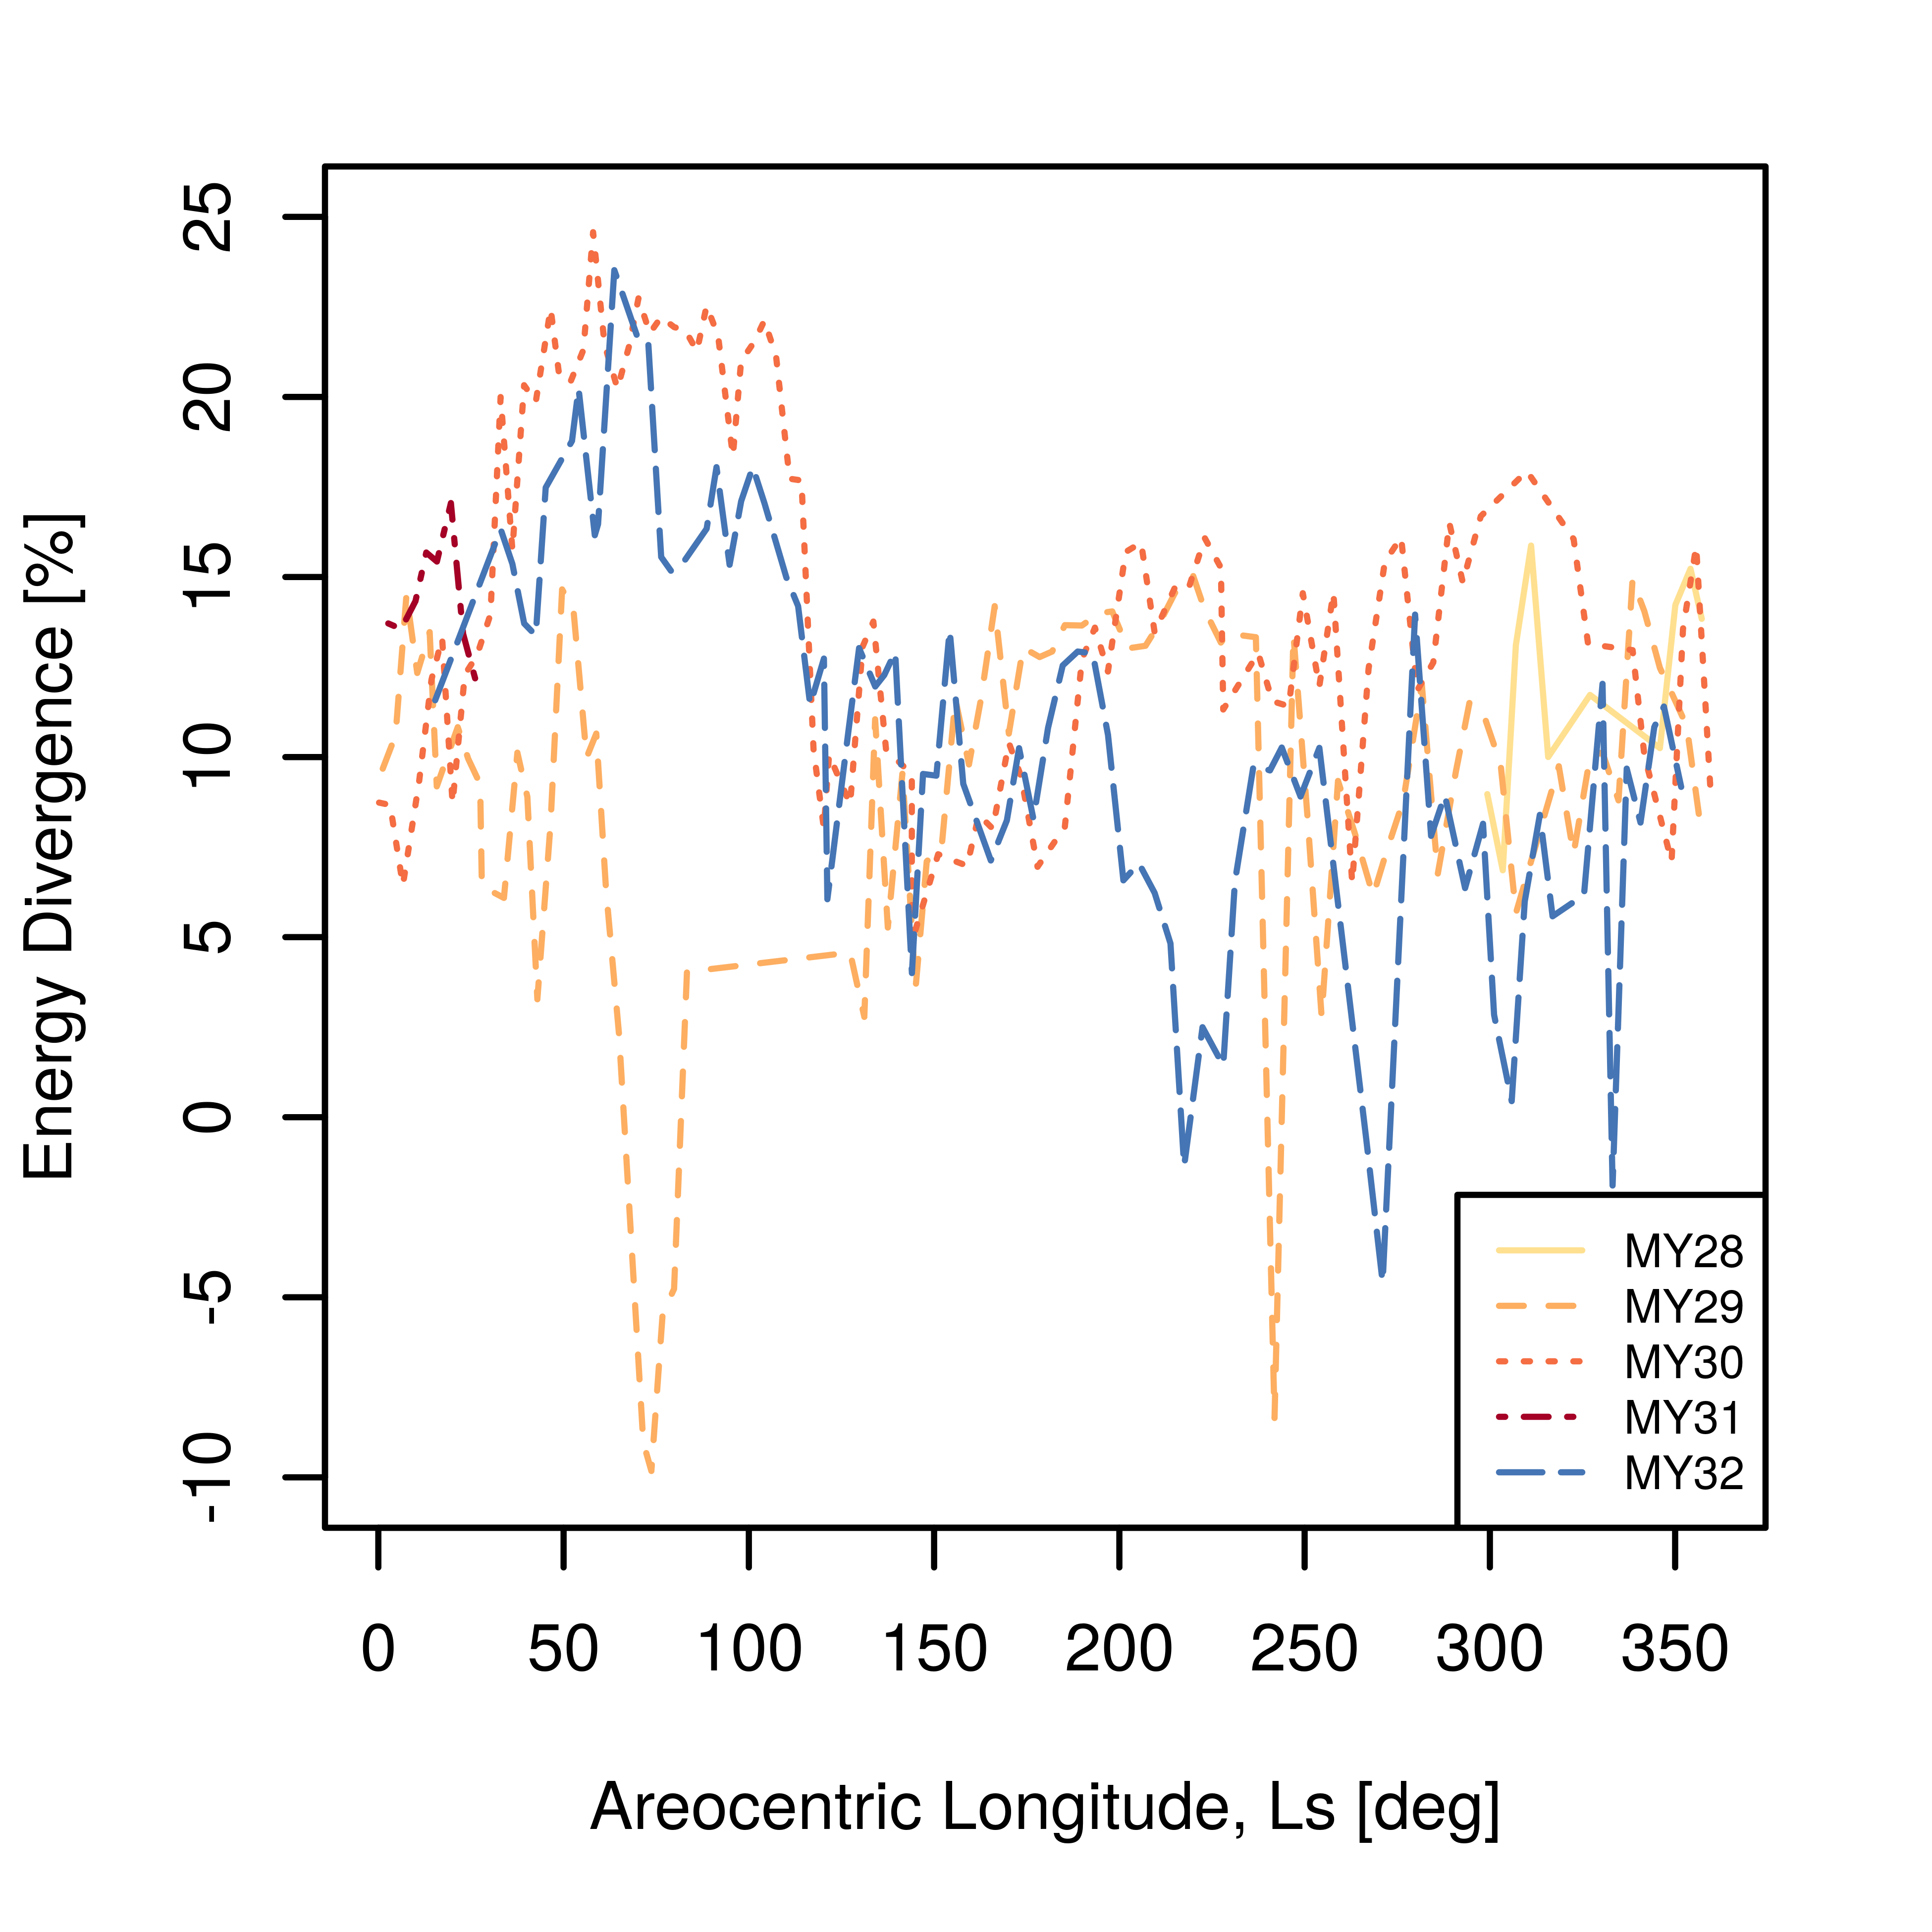
\includegraphics[height=\graphicsHeight]{sections/appendix/energy-error-margin/plots/energy-prediction-divergences-from-my28-to-my32-adjusted.png}
            \subcaption{Including outliers}
            \label{fig:plot:mer-energy-prediction-divergences-adjusted-including-outliers}
    \end{subfigure}\hfill
    \begin{subfigure}[t]{\subfigureWidth}
        \centering
            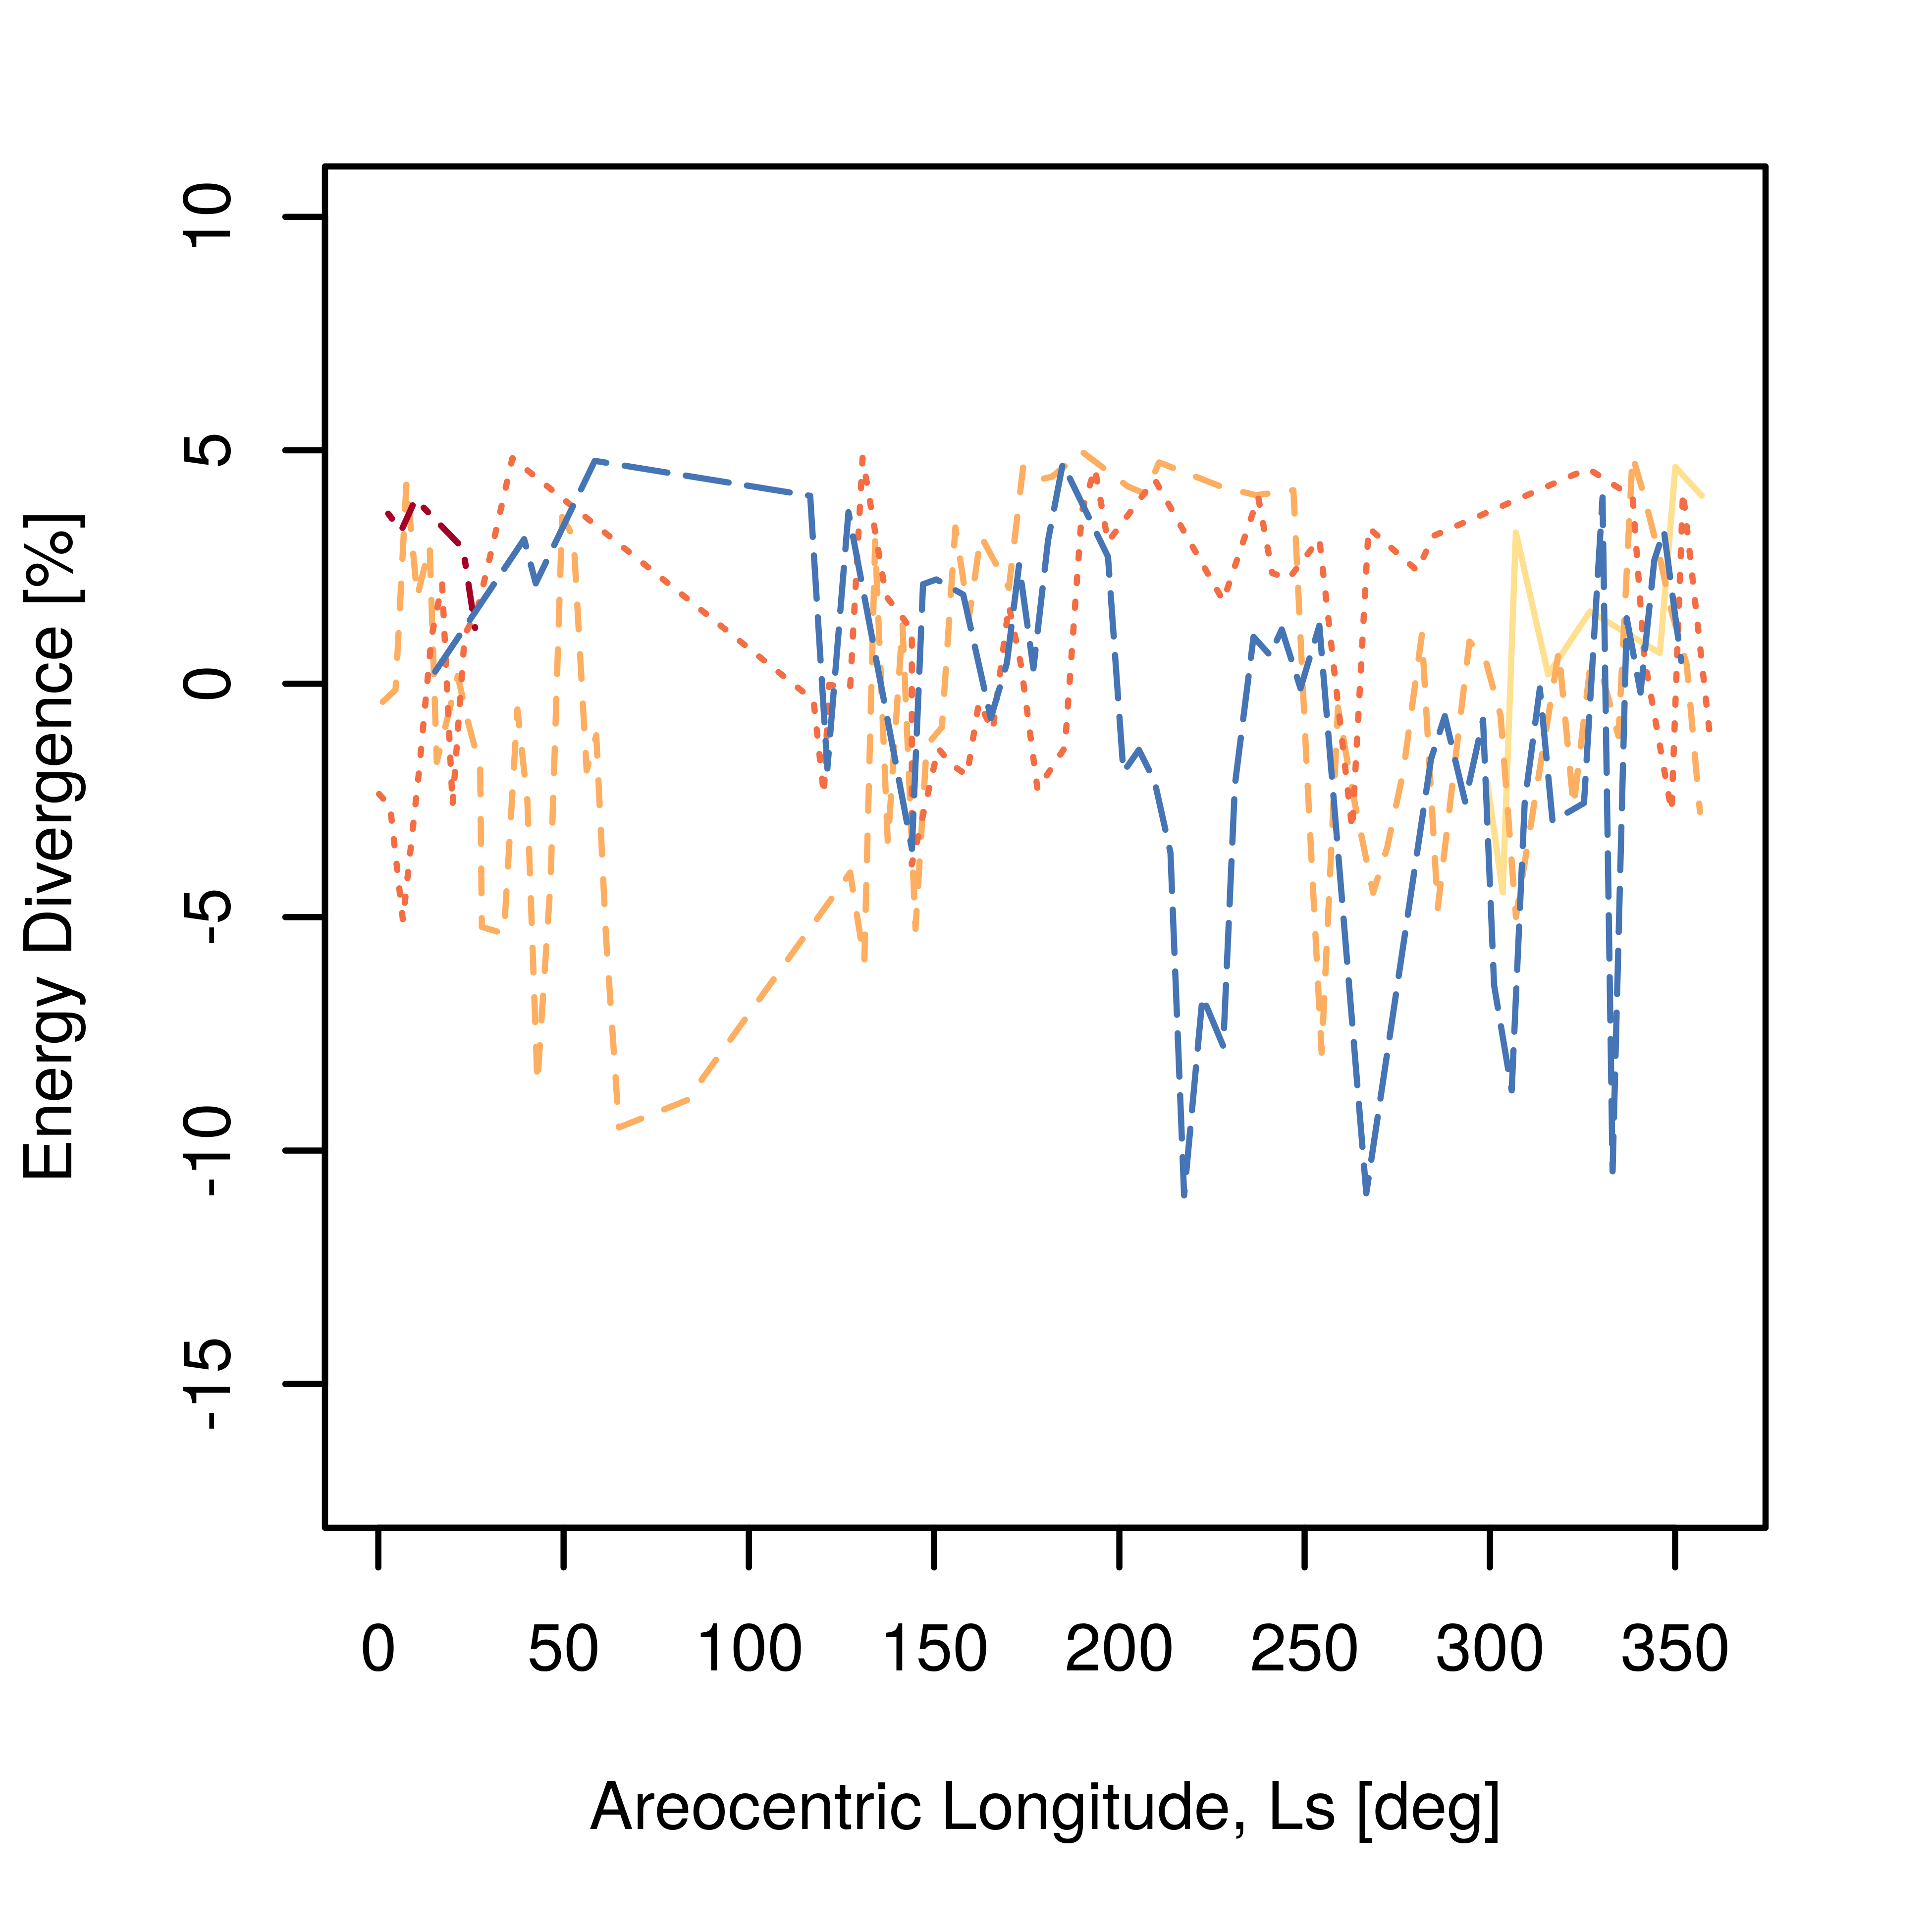
\includegraphics[height=\graphicsHeight]{sections/appendix/energy-error-margin/plots/energy-prediction-divergences-from-my28-to-my32-adjusted-without-outliers.png}
            \subcaption{Ignoring outliers}
            \label{fig:plot:mer-energy-prediction-divergences-adjusted-without-outliers}
    \end{subfigure}\\[0.8ex]
    \caption[Adjusted divergences from energy measured by Opportunity]
    {Adjusted divergences from energy measured by Opportunity.}
    \label{fig:plot:mer-energy-prediction-divergences-adjusted}
\vspace{-2ex}
\end{figure}

\begin{table}[h]
\centering
\caption{Combination of shadowing and other losses with solar array dust factor adjustment coefficients to obtain different error margin ranges. }
\label{tab:target-error-margins}
\begin{tabular}{|c|c|c|}
\hline
\textbf{\begin{tabular}[c]{@{}c@{}}Error\\ Margins\\ Ranges\end{tabular}} & \textbf{\begin{tabular}[c]{@{}c@{}}Shadowing\\ and\\ Other Losses\end{tabular}} & \textbf{\begin{tabular}[c]{@{}c@{}}Solar Array\\ Dust Factor\\ Adjustment\end{tabular}} \\ \hline
\multirow{3}{*}{-20\% / +18\%} & 5\% & 7.5\% \\ \cline{2-3}
 & 6\% & 5.5\% \\ \cline{2-3}
 & 7\% & 3.5\% \\ \hhline{|=|=|=|}
\multirow{3}{*}{-15\% / +21\%} & 5\% & 10.3\% \\ \cline{2-3}
 & 6\% & 8.3\% \\ \cline{2-3}
 & 7\% & 6.3\% \\ \hhline{|=|=|=|}
\multirow{3}{*}{-14\% / +22\%} & 5\% & 10.8\% \\ \cline{2-3}
 & 6\% & 8.8\% \\ \cline{2-3}
 & 7\% & 6.3\% \\ \hhline{|=|=|=|}
\multirow{3}{*}{-13\% / +23\%} & 5\% & 11.4\% \\ \cline{2-3}
 & 6\% & 9.4\% \\ \cline{2-3}
 & 7\% & 7.4\% \\ \hhline{|=|=|=|}
\multirow{3}{*}{-12\% / +23\%} & 5\% & 11.9\% \\ \cline{2-3}
 & 6\% & 9.9\% \\ \cline{2-3}
 & 7\% & 7.9\% \\ \hhline{|=|=|=|}
\multirow{3}{*}{-11\% / +24\%} & 5\% & 12.5\% \\ \cline{2-3}
 & 6\% & 10.5\% \\ \cline{2-3}
 & 7\% & 8.5\% \\ \hhline{|=|=|=|}
\multirow{3}{*}{-10\% / +25\%} & 5\% & 13.1\% \\ \cline{2-3}
 & 6\% & 11.1\% \\ \cline{2-3}
 & 7\% & 9.1\% \\ \hline
\end{tabular}
\end{table}


\section{Ignoring Outliers}
\label{sec:Appendix:NarrowedEnergyPredictionErrorMarginRange:IgnoringOutliers}

In \refFig{fig:plot:binned-error-margins}, divergences greater than \SI{5}{\percent} and lesser than \SI{-15}{\percent} are obtained with only \SI{9.2}{\percent} of the dataset. With this in consideration, the process described in \refSec{sec:Appendix:NarrowedEnergyPredictionErrorMarginRange:PreservingOutliers} is repeated without the data points responsible for the divergence outliers. This further narrows down the error margin range to \SI{-11}{\percent}/+\SI{5}{\percent} by applying solar array dust factor adjustment of \SI{5.4}{\percent} coupled with shadowing and other losses of \SI{5}{\percent}. The resulting adjusted divergences are presented in \refFig{fig:plot:mer-energy-prediction-divergences-adjusted-without-outliers}:


\section{Result}
\label{sec:Appendix:NarrowedEnergyPredictionErrorMarginRange:Conclusion}

The predicted generated energy curves in \refFig{fig:plot:sub:mer-energy-production-predicted-vs-reported-my29-adjusted}, \refFig{fig:plot:sub:mer-energy-production-predicted-vs-reported-my30-adjusted}, and \refFig{fig:plot:sub:mer-energy-production-predicted-vs-reported-my32-adjusted} are obtained through the process described in \refSec{sec:Appendix:NarrowedEnergyPredictionErrorMarginRange:PreservingOutliers}. This resulted in overly conservative predictions when compared with the curve representing energy productions reported by MER Opportunity. Predictions in \refFig{fig:plot:sub:mer-energy-production-predicted-vs-reported-my29-adjusted-without-outliers}, \refFig{fig:plot:sub:mer-energy-production-predicted-vs-reported-my30-adjusted-without-outliers}, and \refFig{fig:plot:sub:mer-energy-production-predicted-vs-reported-my32-adjusted-without-outliers} are obtained through the process described in \refSec{sec:Appendix:NarrowedEnergyPredictionErrorMarginRange:IgnoringOutliers}. This results predictions that more closely follow the reported energy productions. Comparing these predictions with the unadjusted values presented in \refFig{fig:plot:mer-energy-production-predicted-vs-reported} shows little changes and therefor do not justify the need to narrow down the error margin range for the purposes of preliminary mission scenario analysis.

\begin{figure}[h]
\captionsetup[subfigure]{justification=centering}
\vspace{-2ex}
	\centering
    %% setup sizes
    \setlength{\subfigureWidth}{0.32\textwidth}
    \setlength{\graphicsHeight}{50mm}
    %% kill hyper-link highlighting
    \hypersetup{hidelinks=true}%
    %% the figures
	\begin{subfigure}[t]{\subfigureWidth}
        \centering
		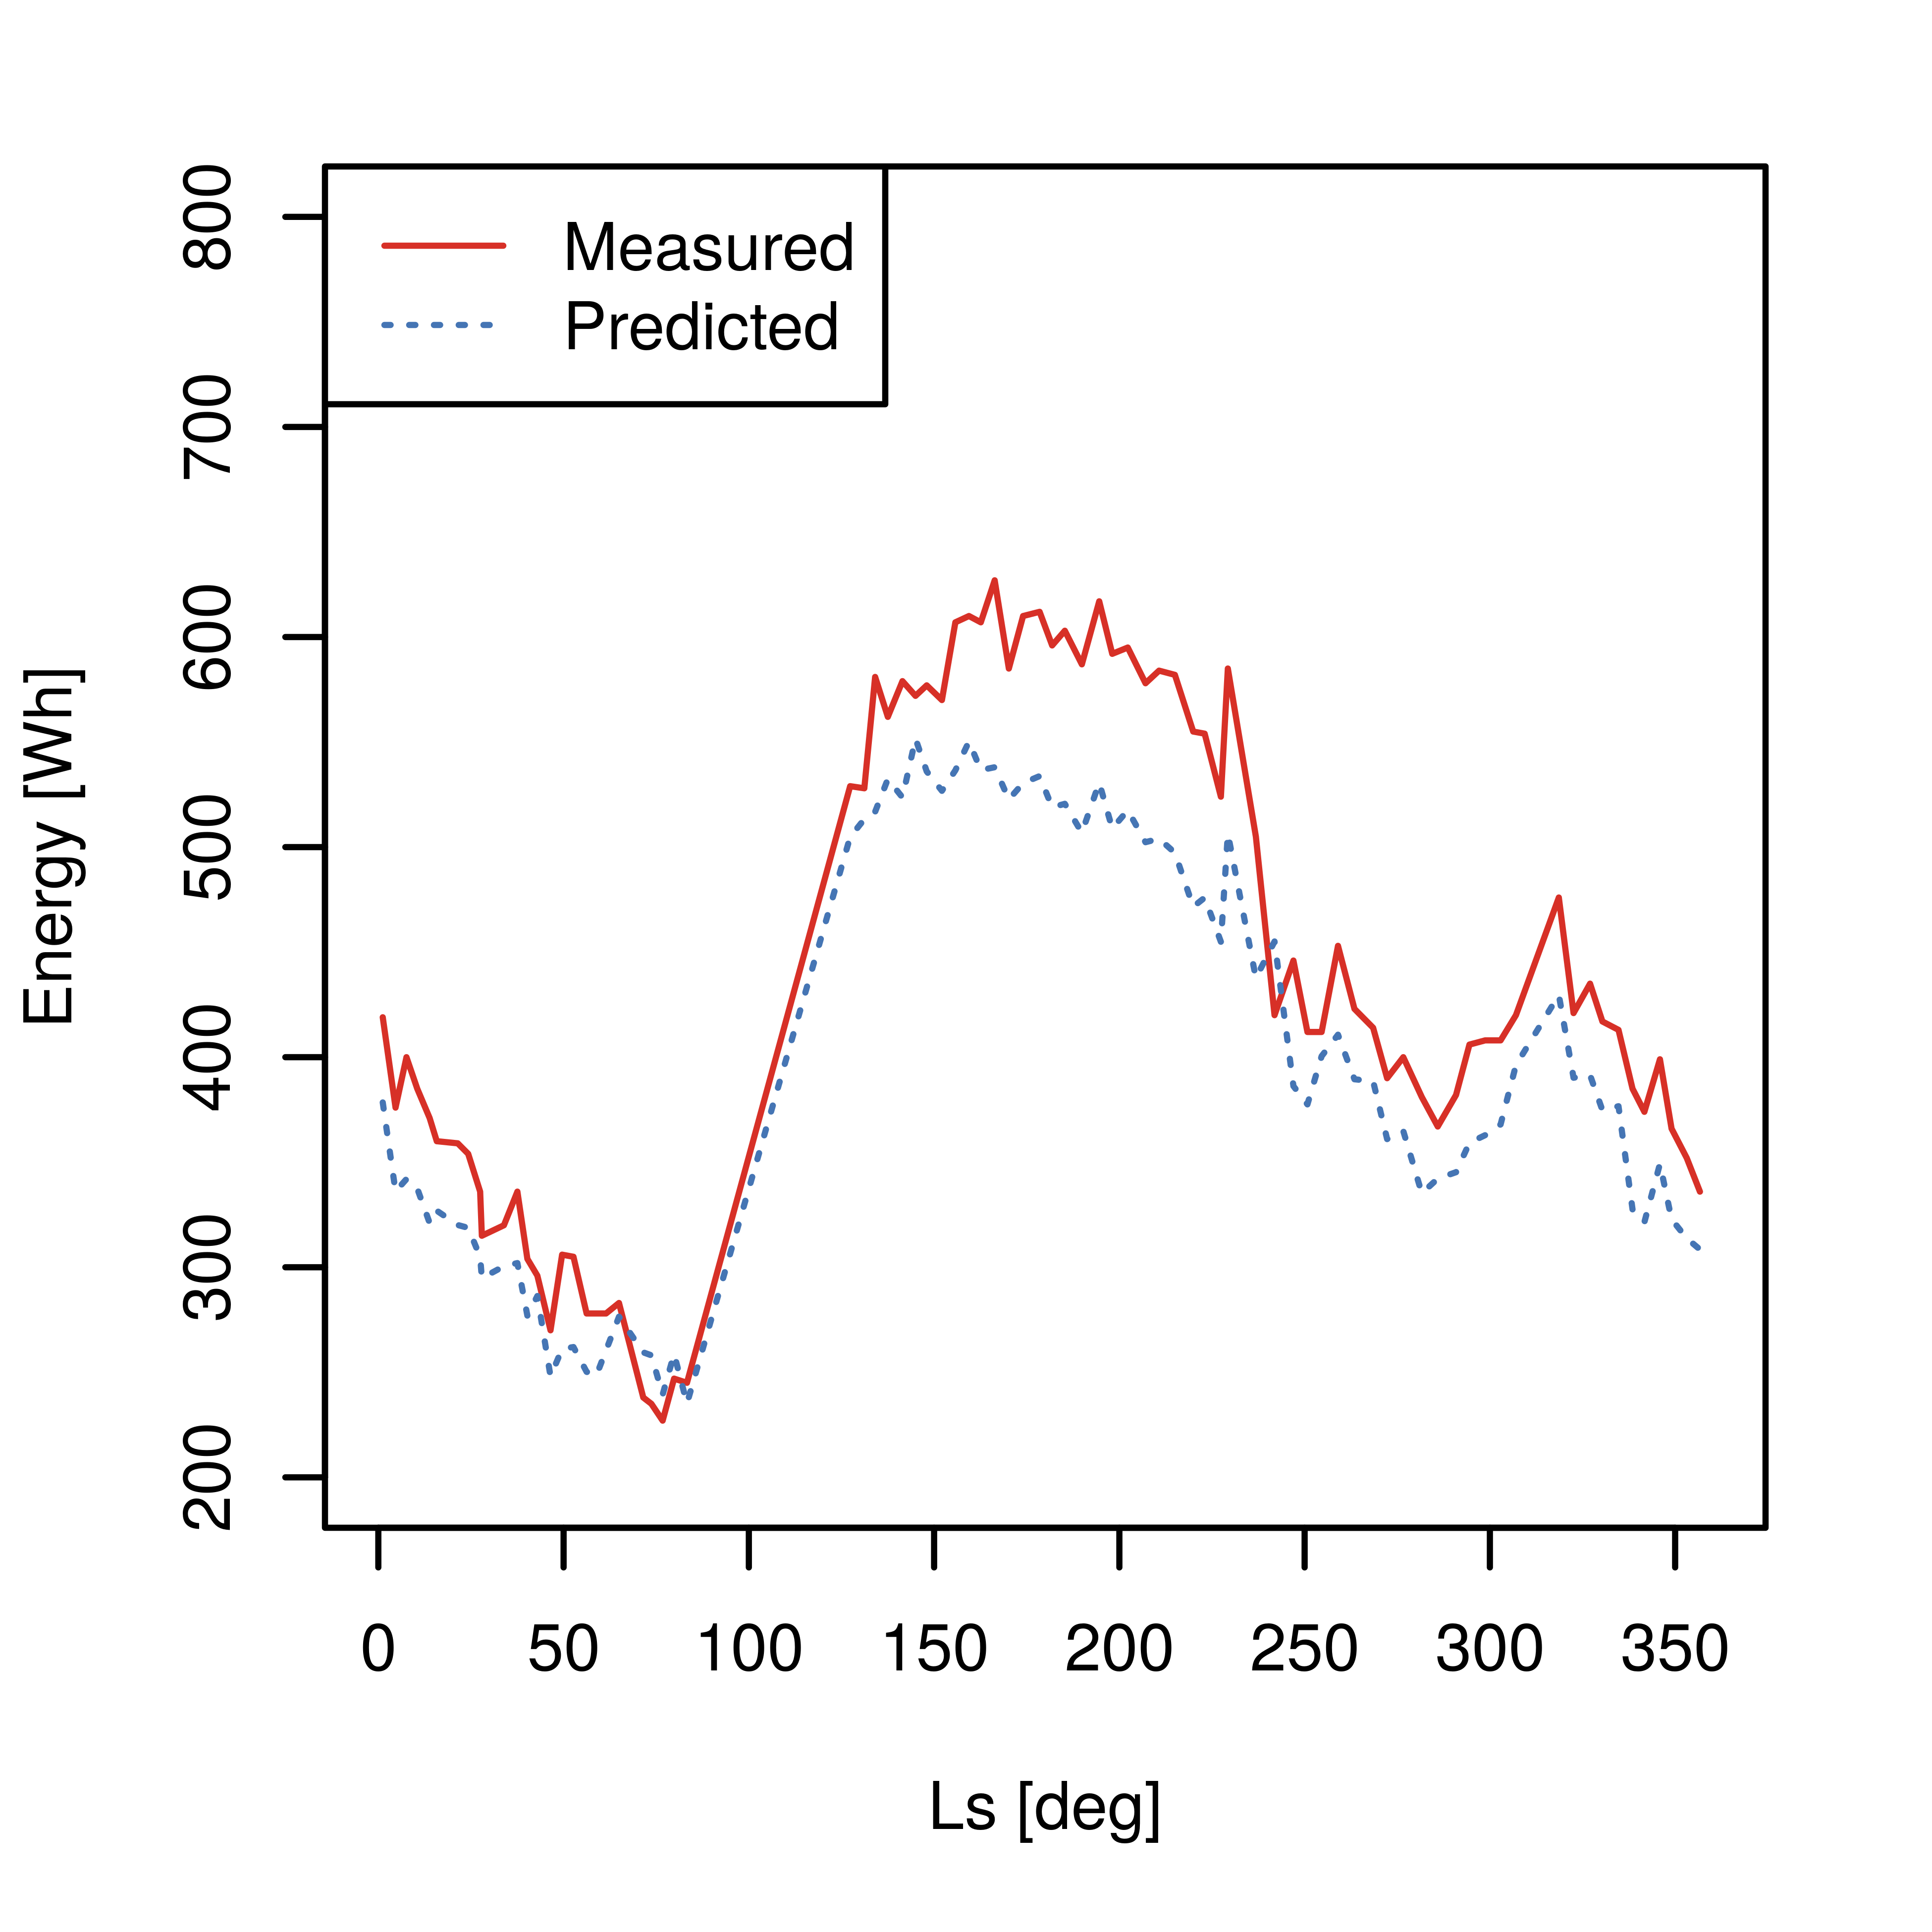
\includegraphics[height=\graphicsHeight]{sections/appendix/energy-error-margin/plots/predicted-vs-measured-energy-my29-adjusted.png}
		\subcaption{MY29 (outliers included)}
		\label{fig:plot:sub:mer-energy-production-predicted-vs-reported-my29-adjusted}
	\end{subfigure}\hfill
	\begin{subfigure}[t]{\subfigureWidth}
        \centering
		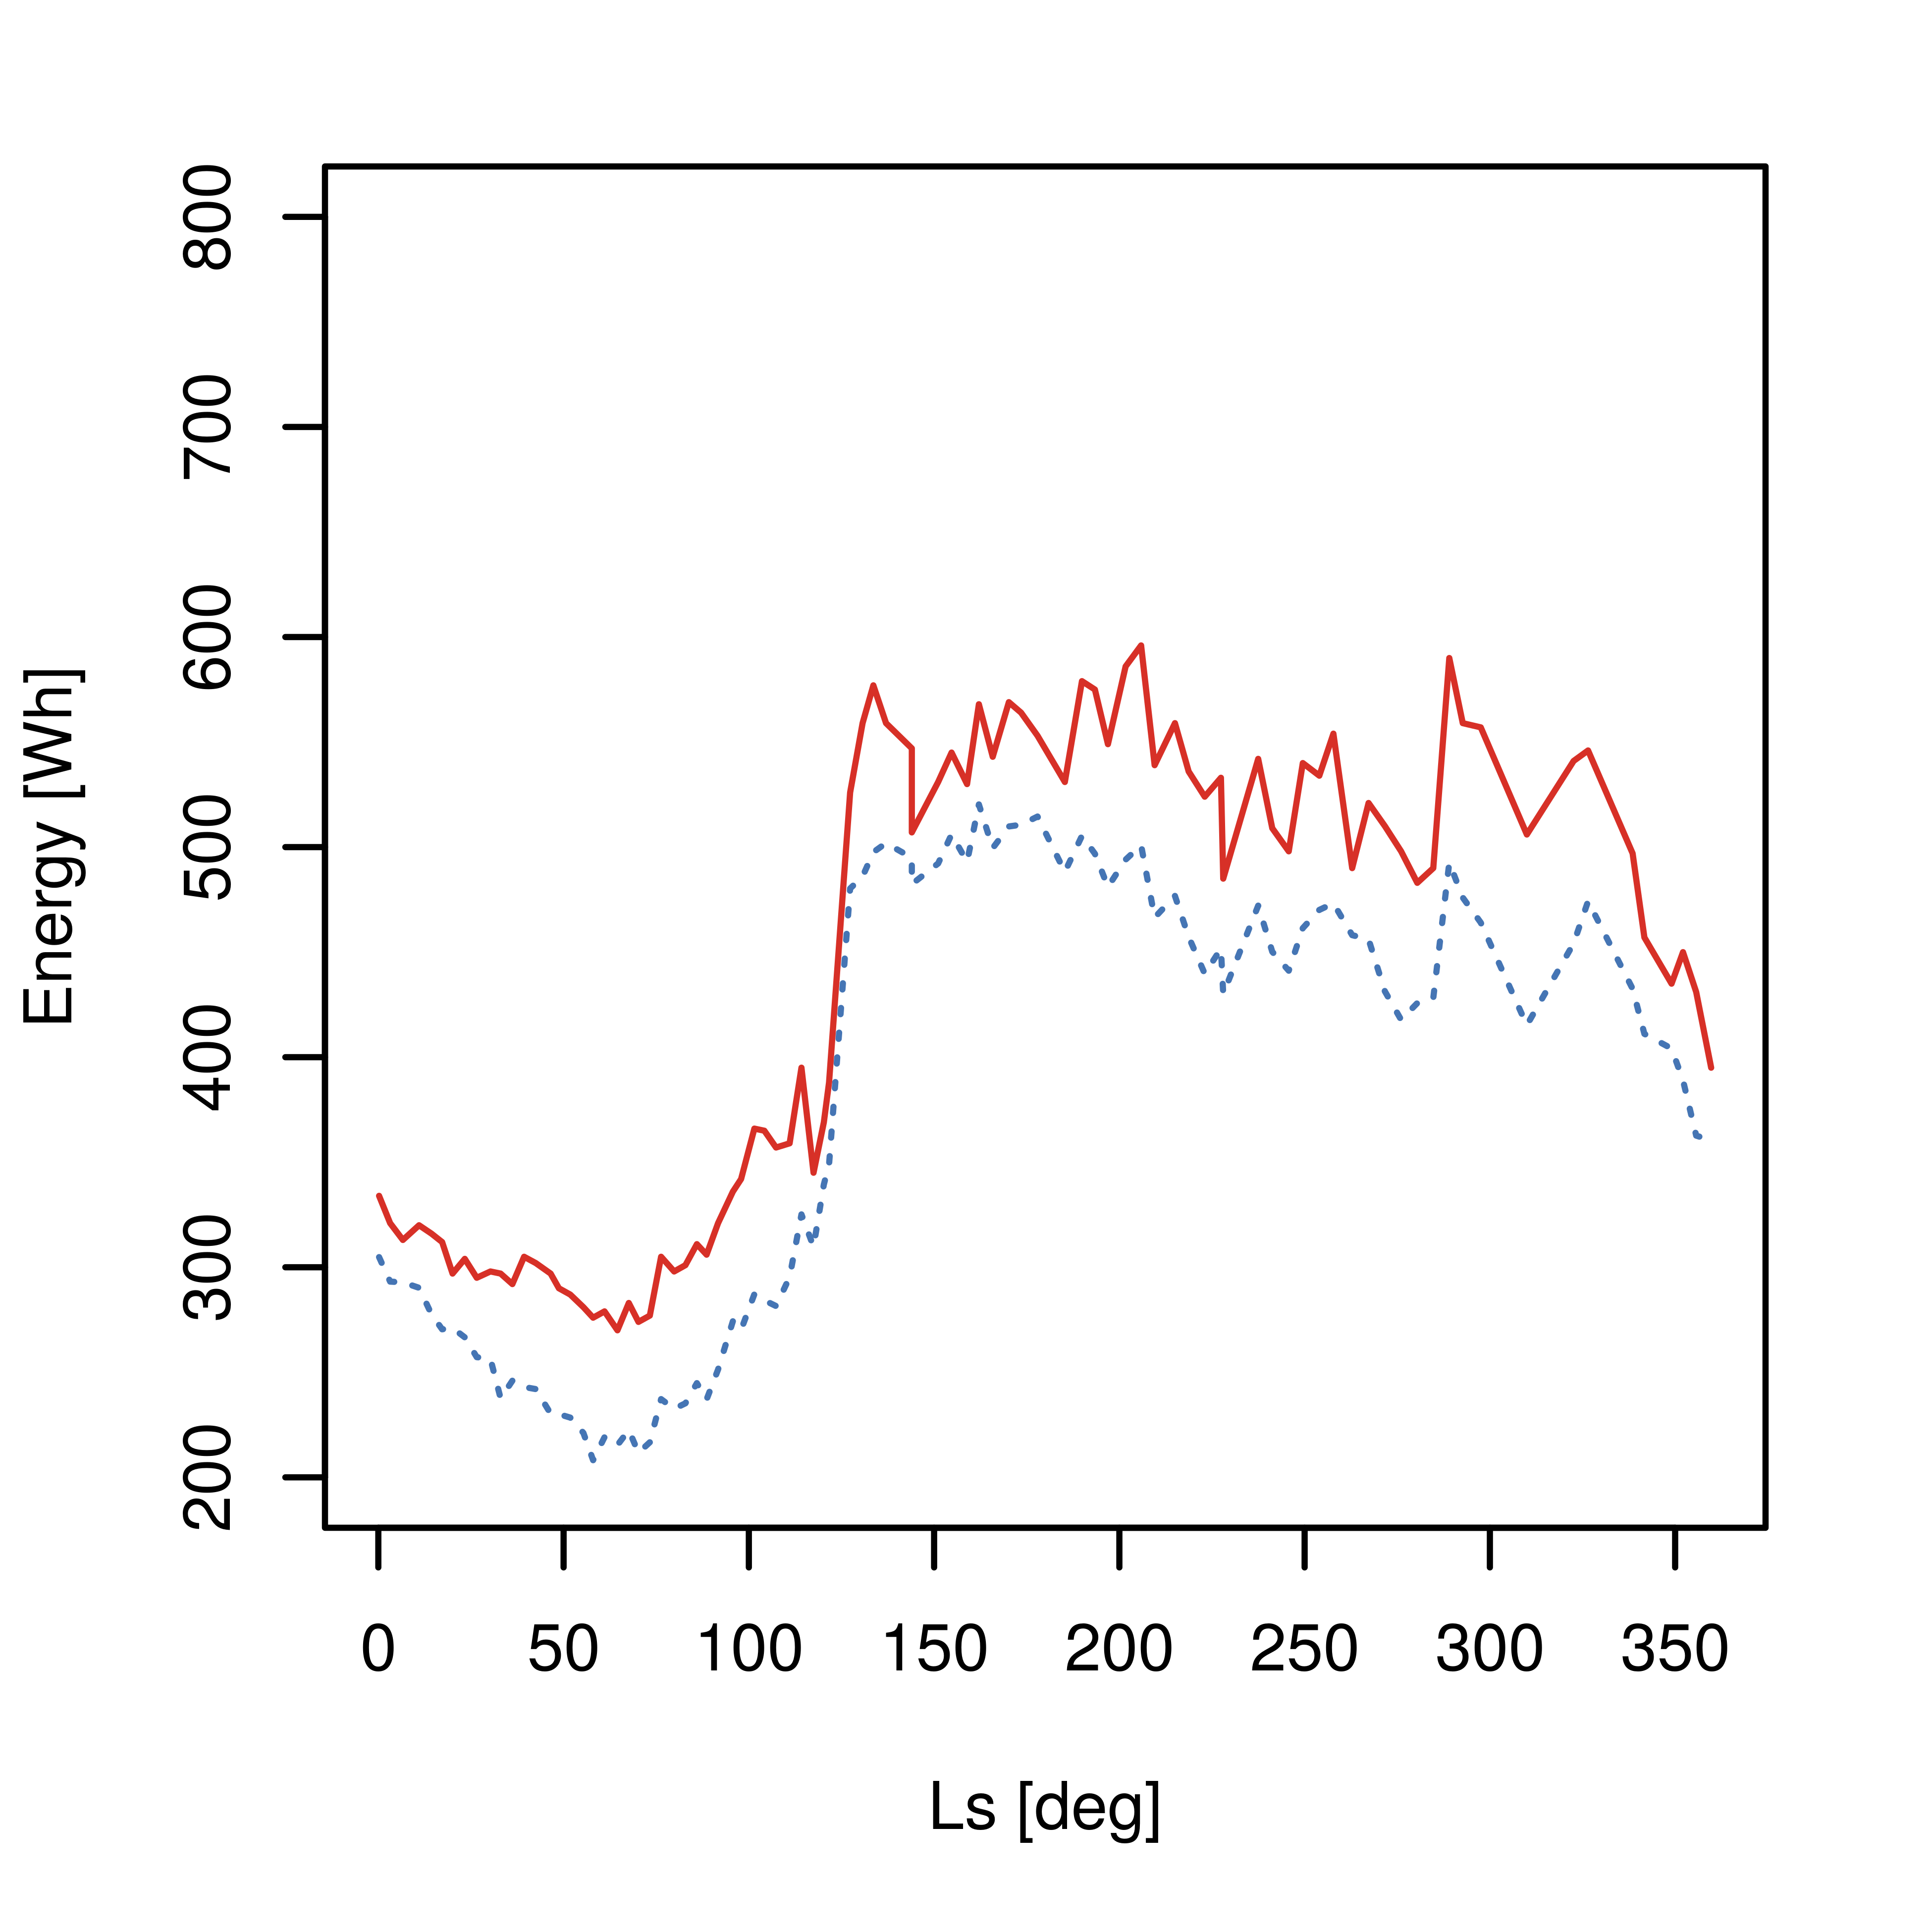
\includegraphics[height=\graphicsHeight]{sections/appendix/energy-error-margin/plots/predicted-vs-measured-energy-my30-adjusted.png}
		\subcaption{MY30 (outliers included)}
		\label{fig:plot:sub:mer-energy-production-predicted-vs-reported-my30-adjusted}
	\end{subfigure}\hfill
    \begin{subfigure}[t]{\subfigureWidth}
        \centering
		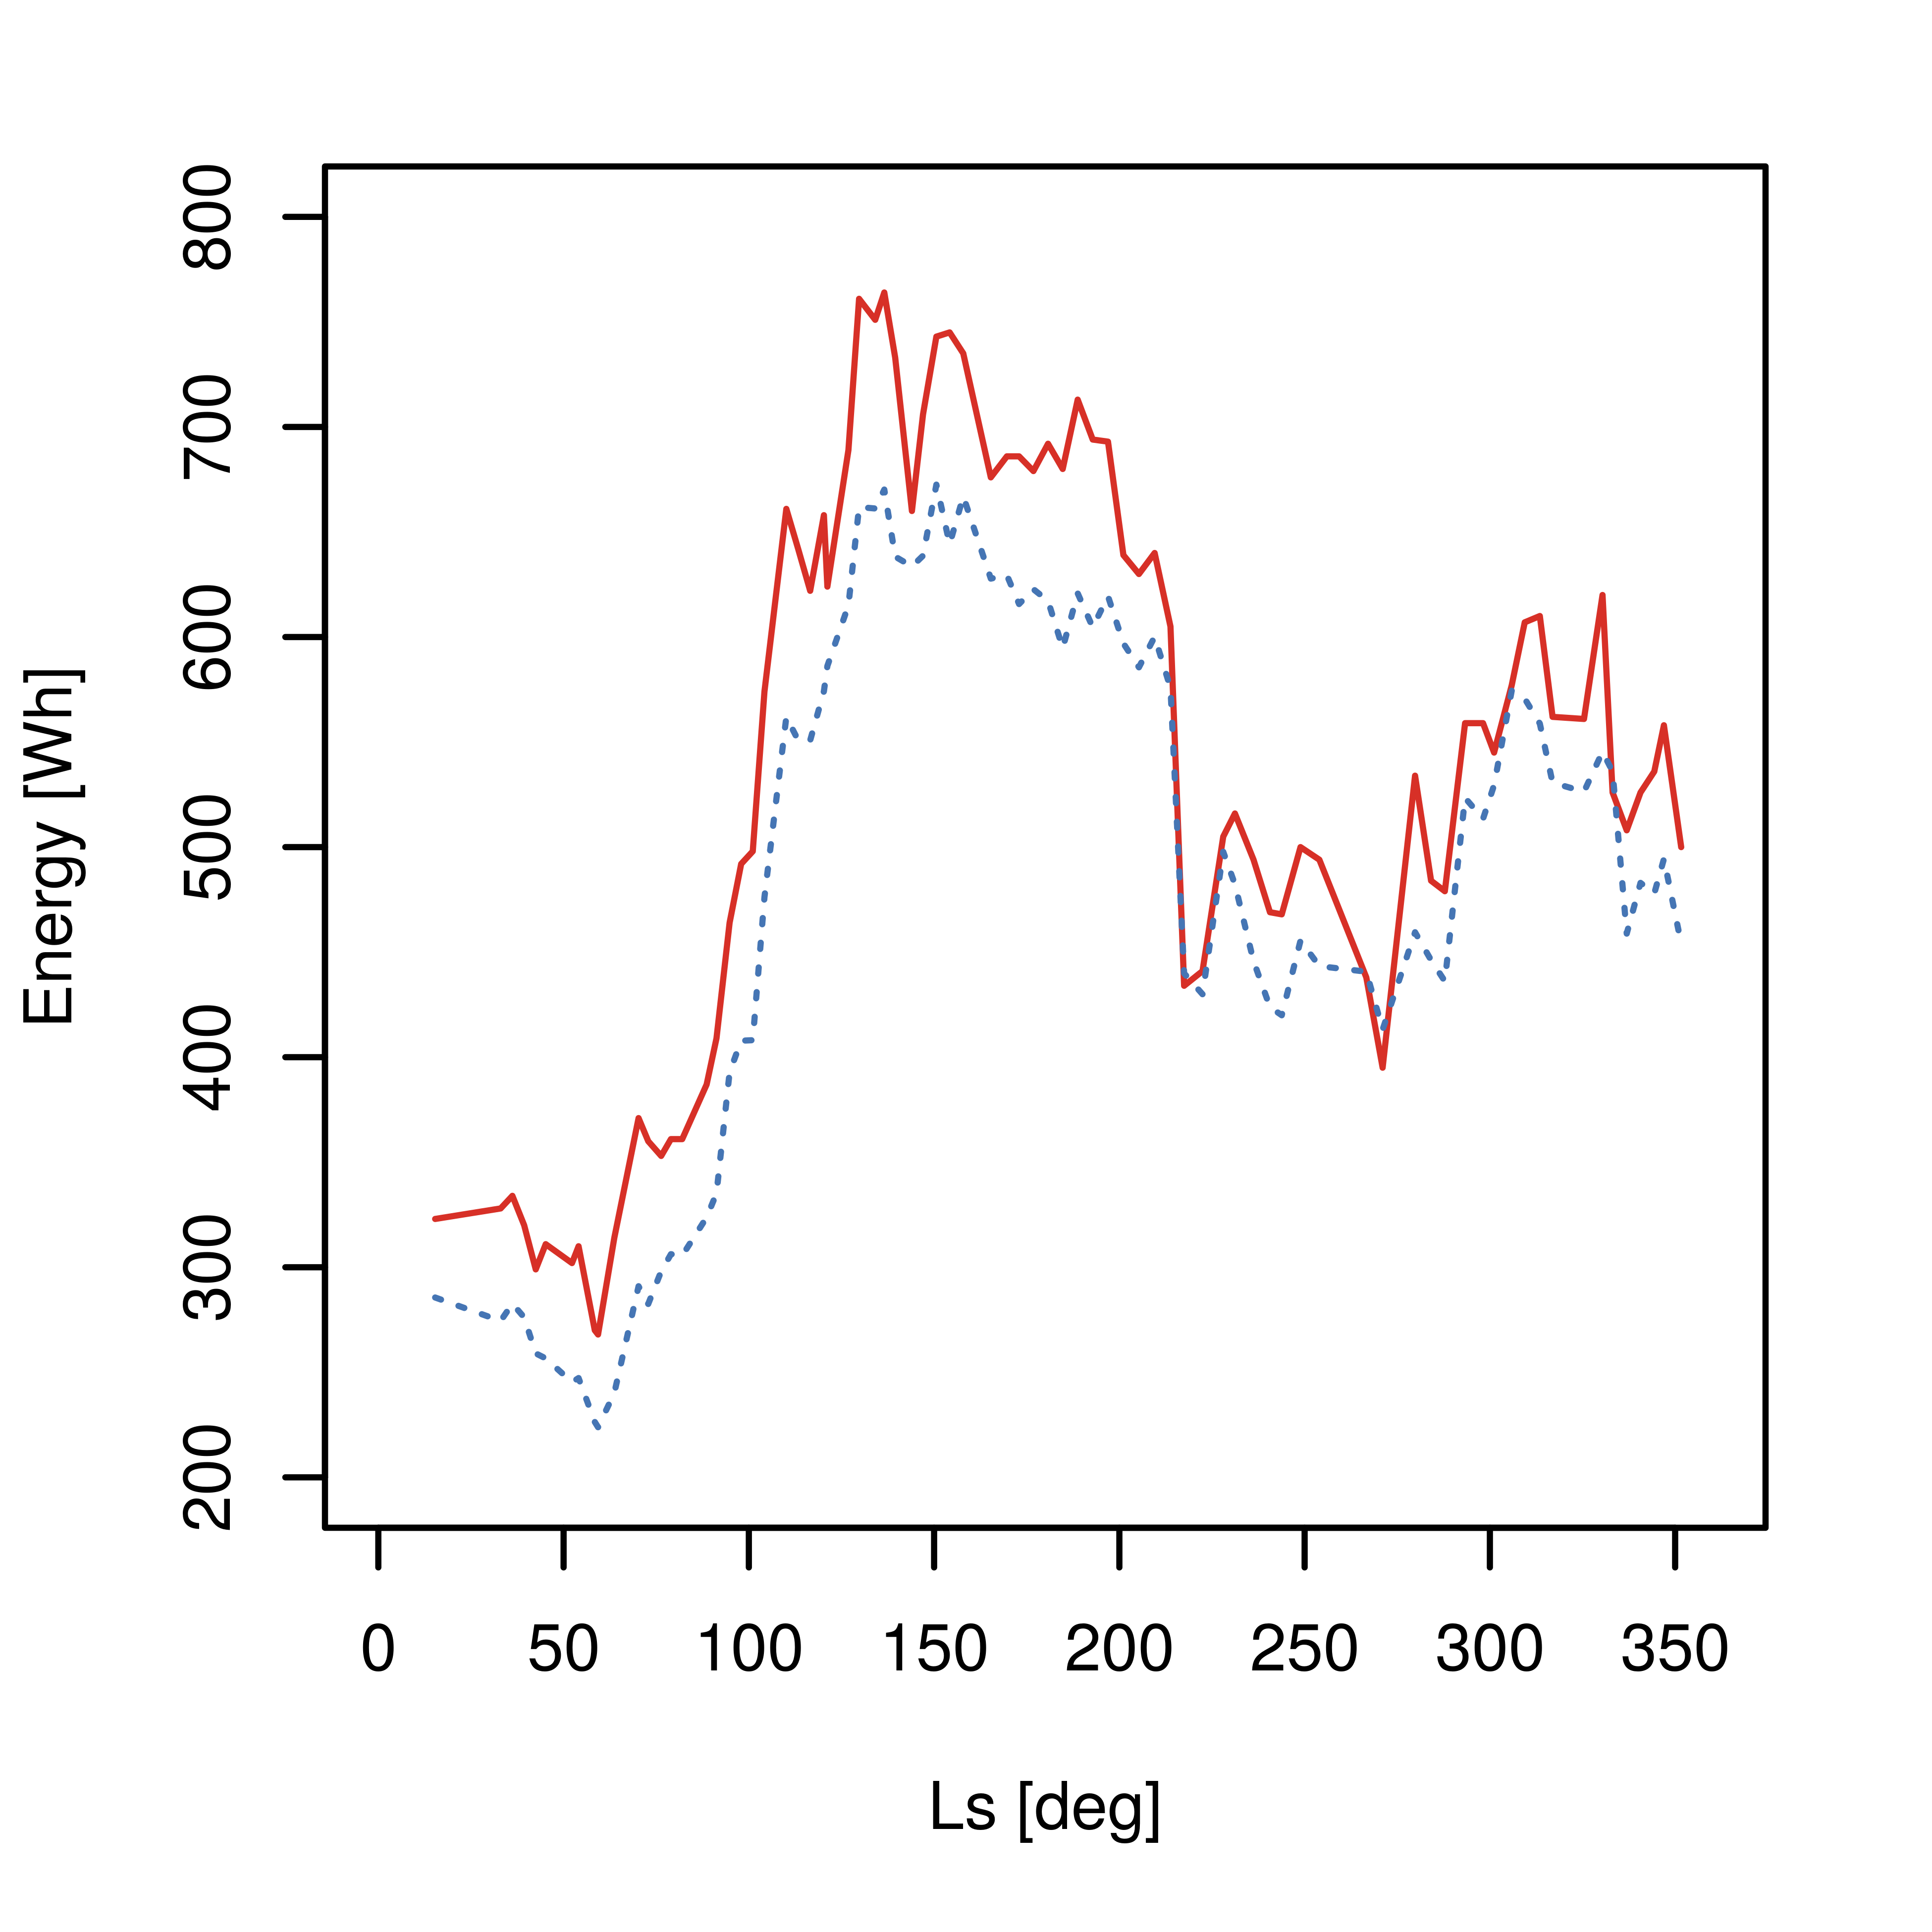
\includegraphics[height=\graphicsHeight]{sections/appendix/energy-error-margin/plots/predicted-vs-measured-energy-my32-adjusted.png}
		\subcaption{MY32 (outliers included)}
		\label{fig:plot:sub:mer-energy-production-predicted-vs-reported-my32-adjusted}
	\end{subfigure}\\[0.8ex]
%% 2nd row
    \begin{subfigure}[t]{\subfigureWidth}
        \centering
		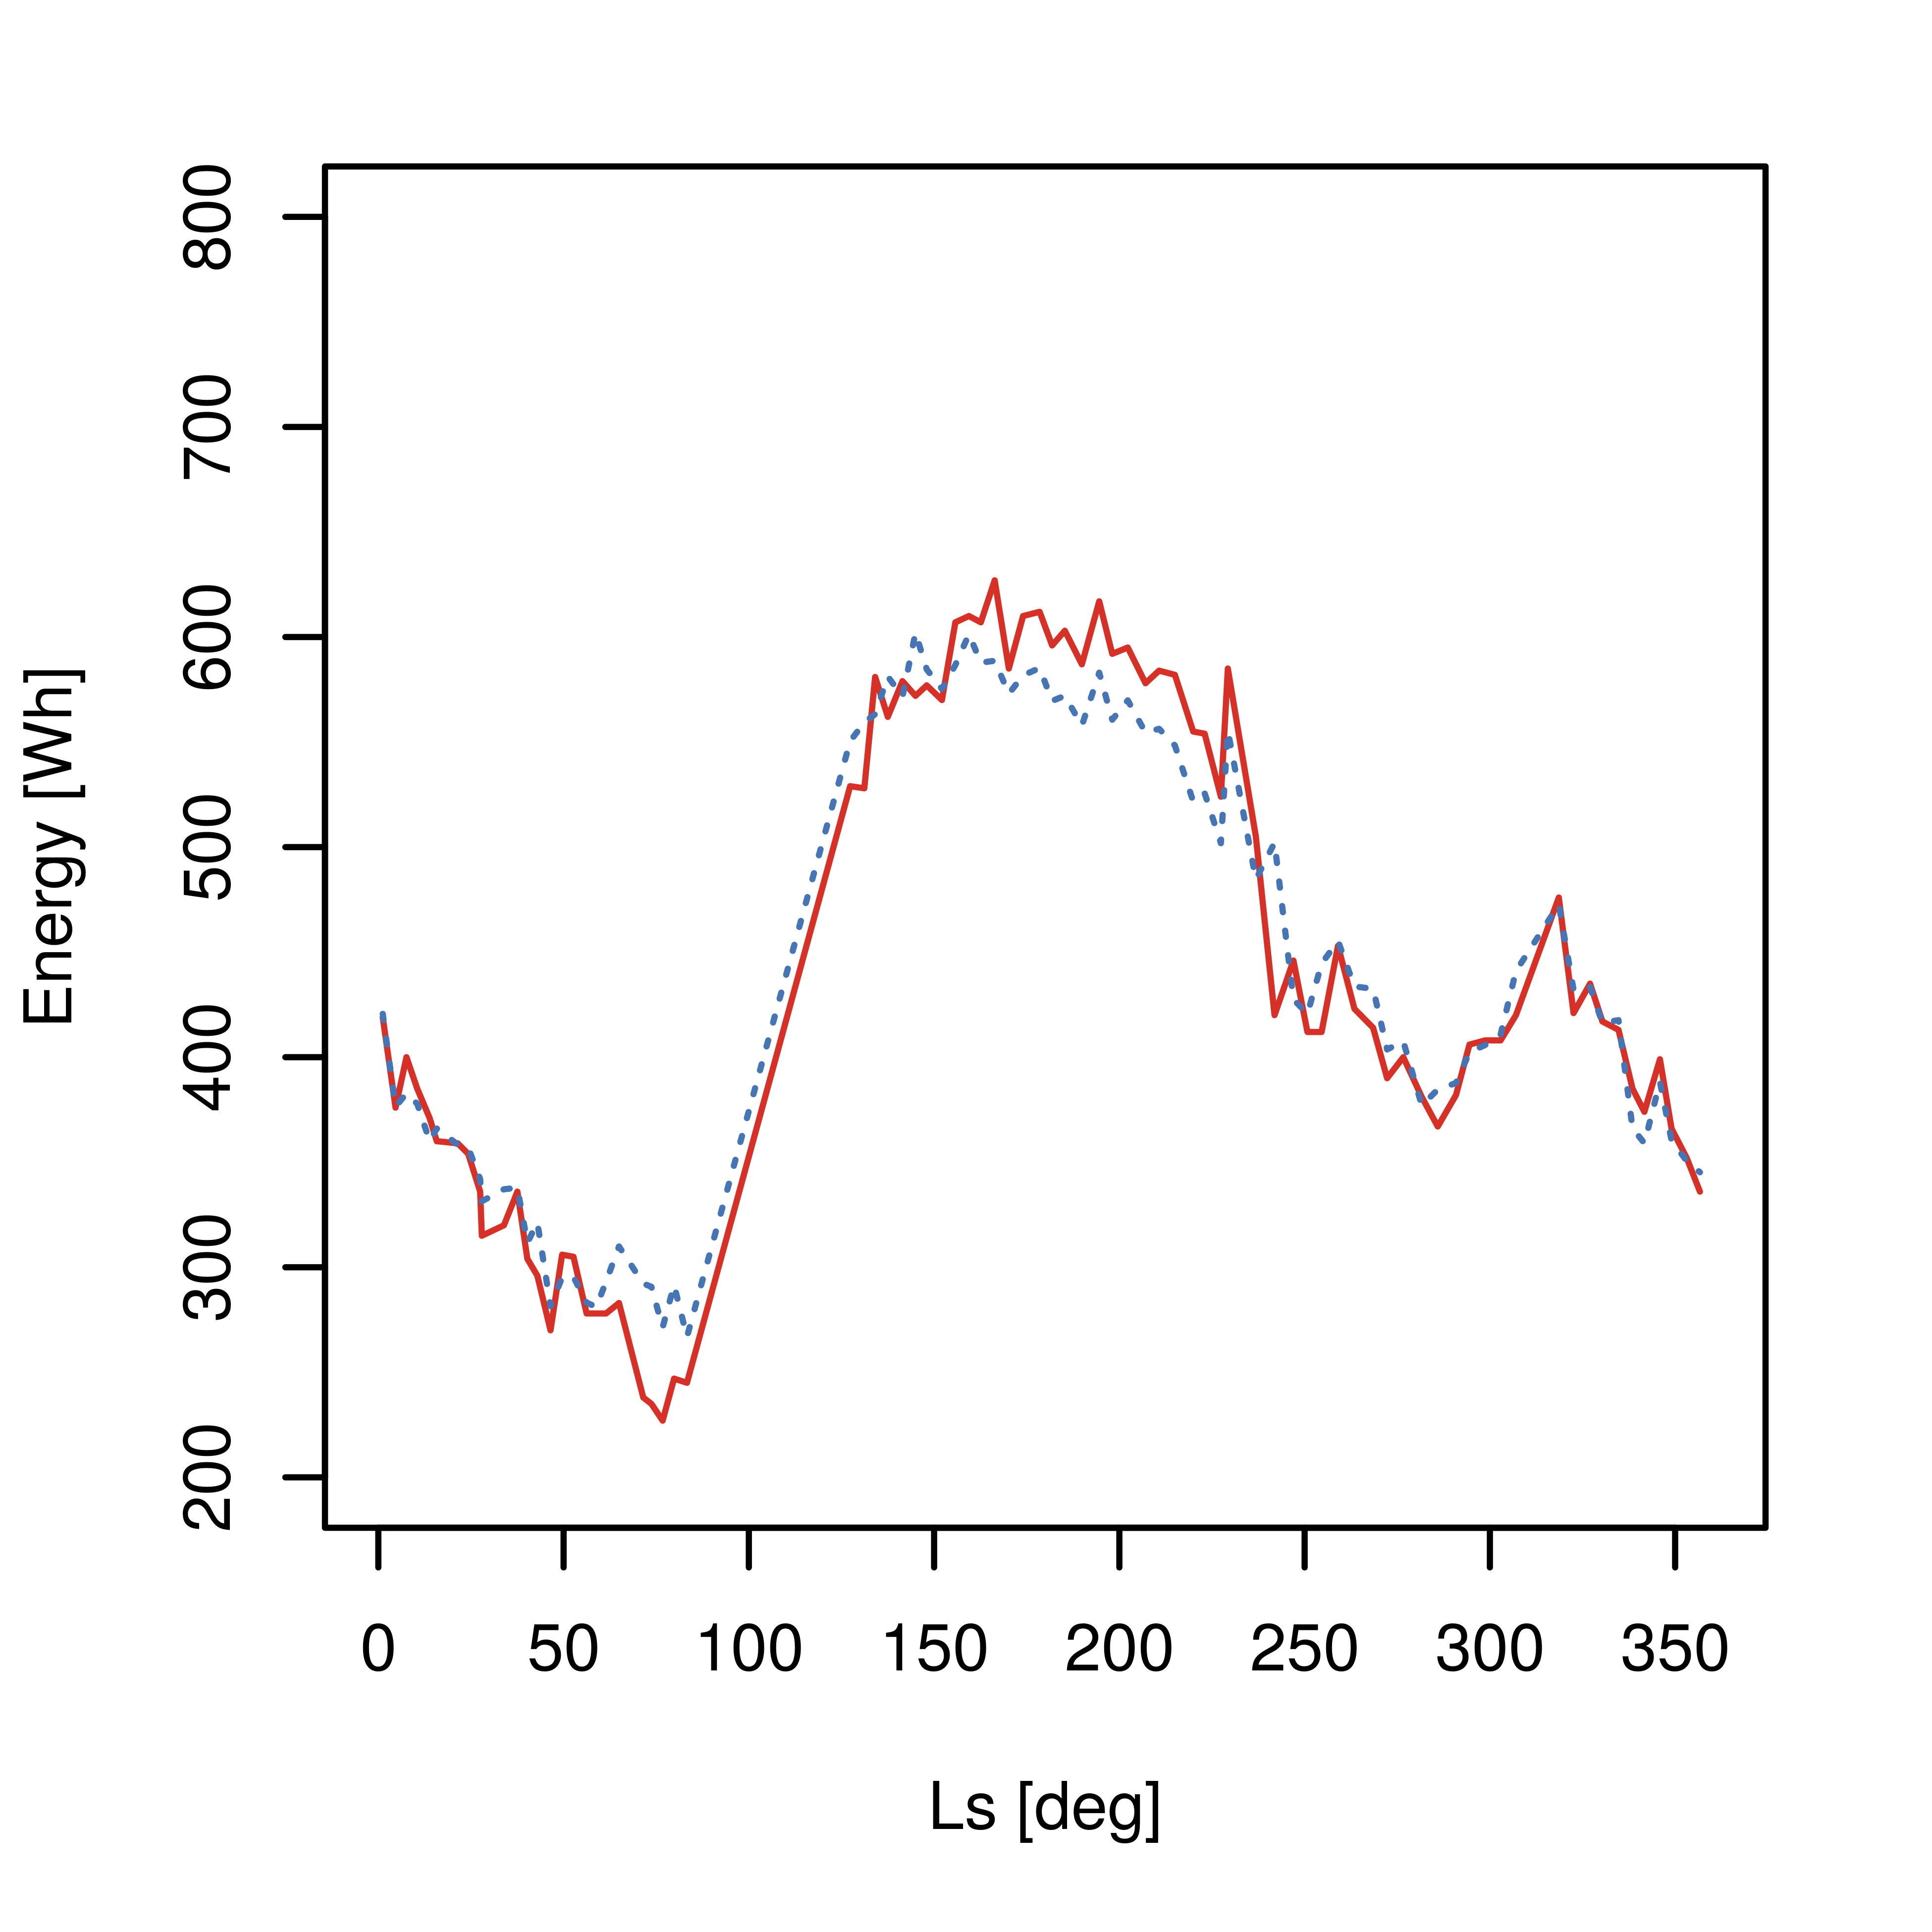
\includegraphics[height=\graphicsHeight]{sections/appendix/energy-error-margin/plots/predicted-vs-measured-energy-my29-adjusted-without-outliers.png}
		\subcaption{MY29 (outliers ignored)}
		\label{fig:plot:sub:mer-energy-production-predicted-vs-reported-my29-adjusted-without-outliers}
	\end{subfigure}\hfill
	\begin{subfigure}[t]{\subfigureWidth}
        \centering
		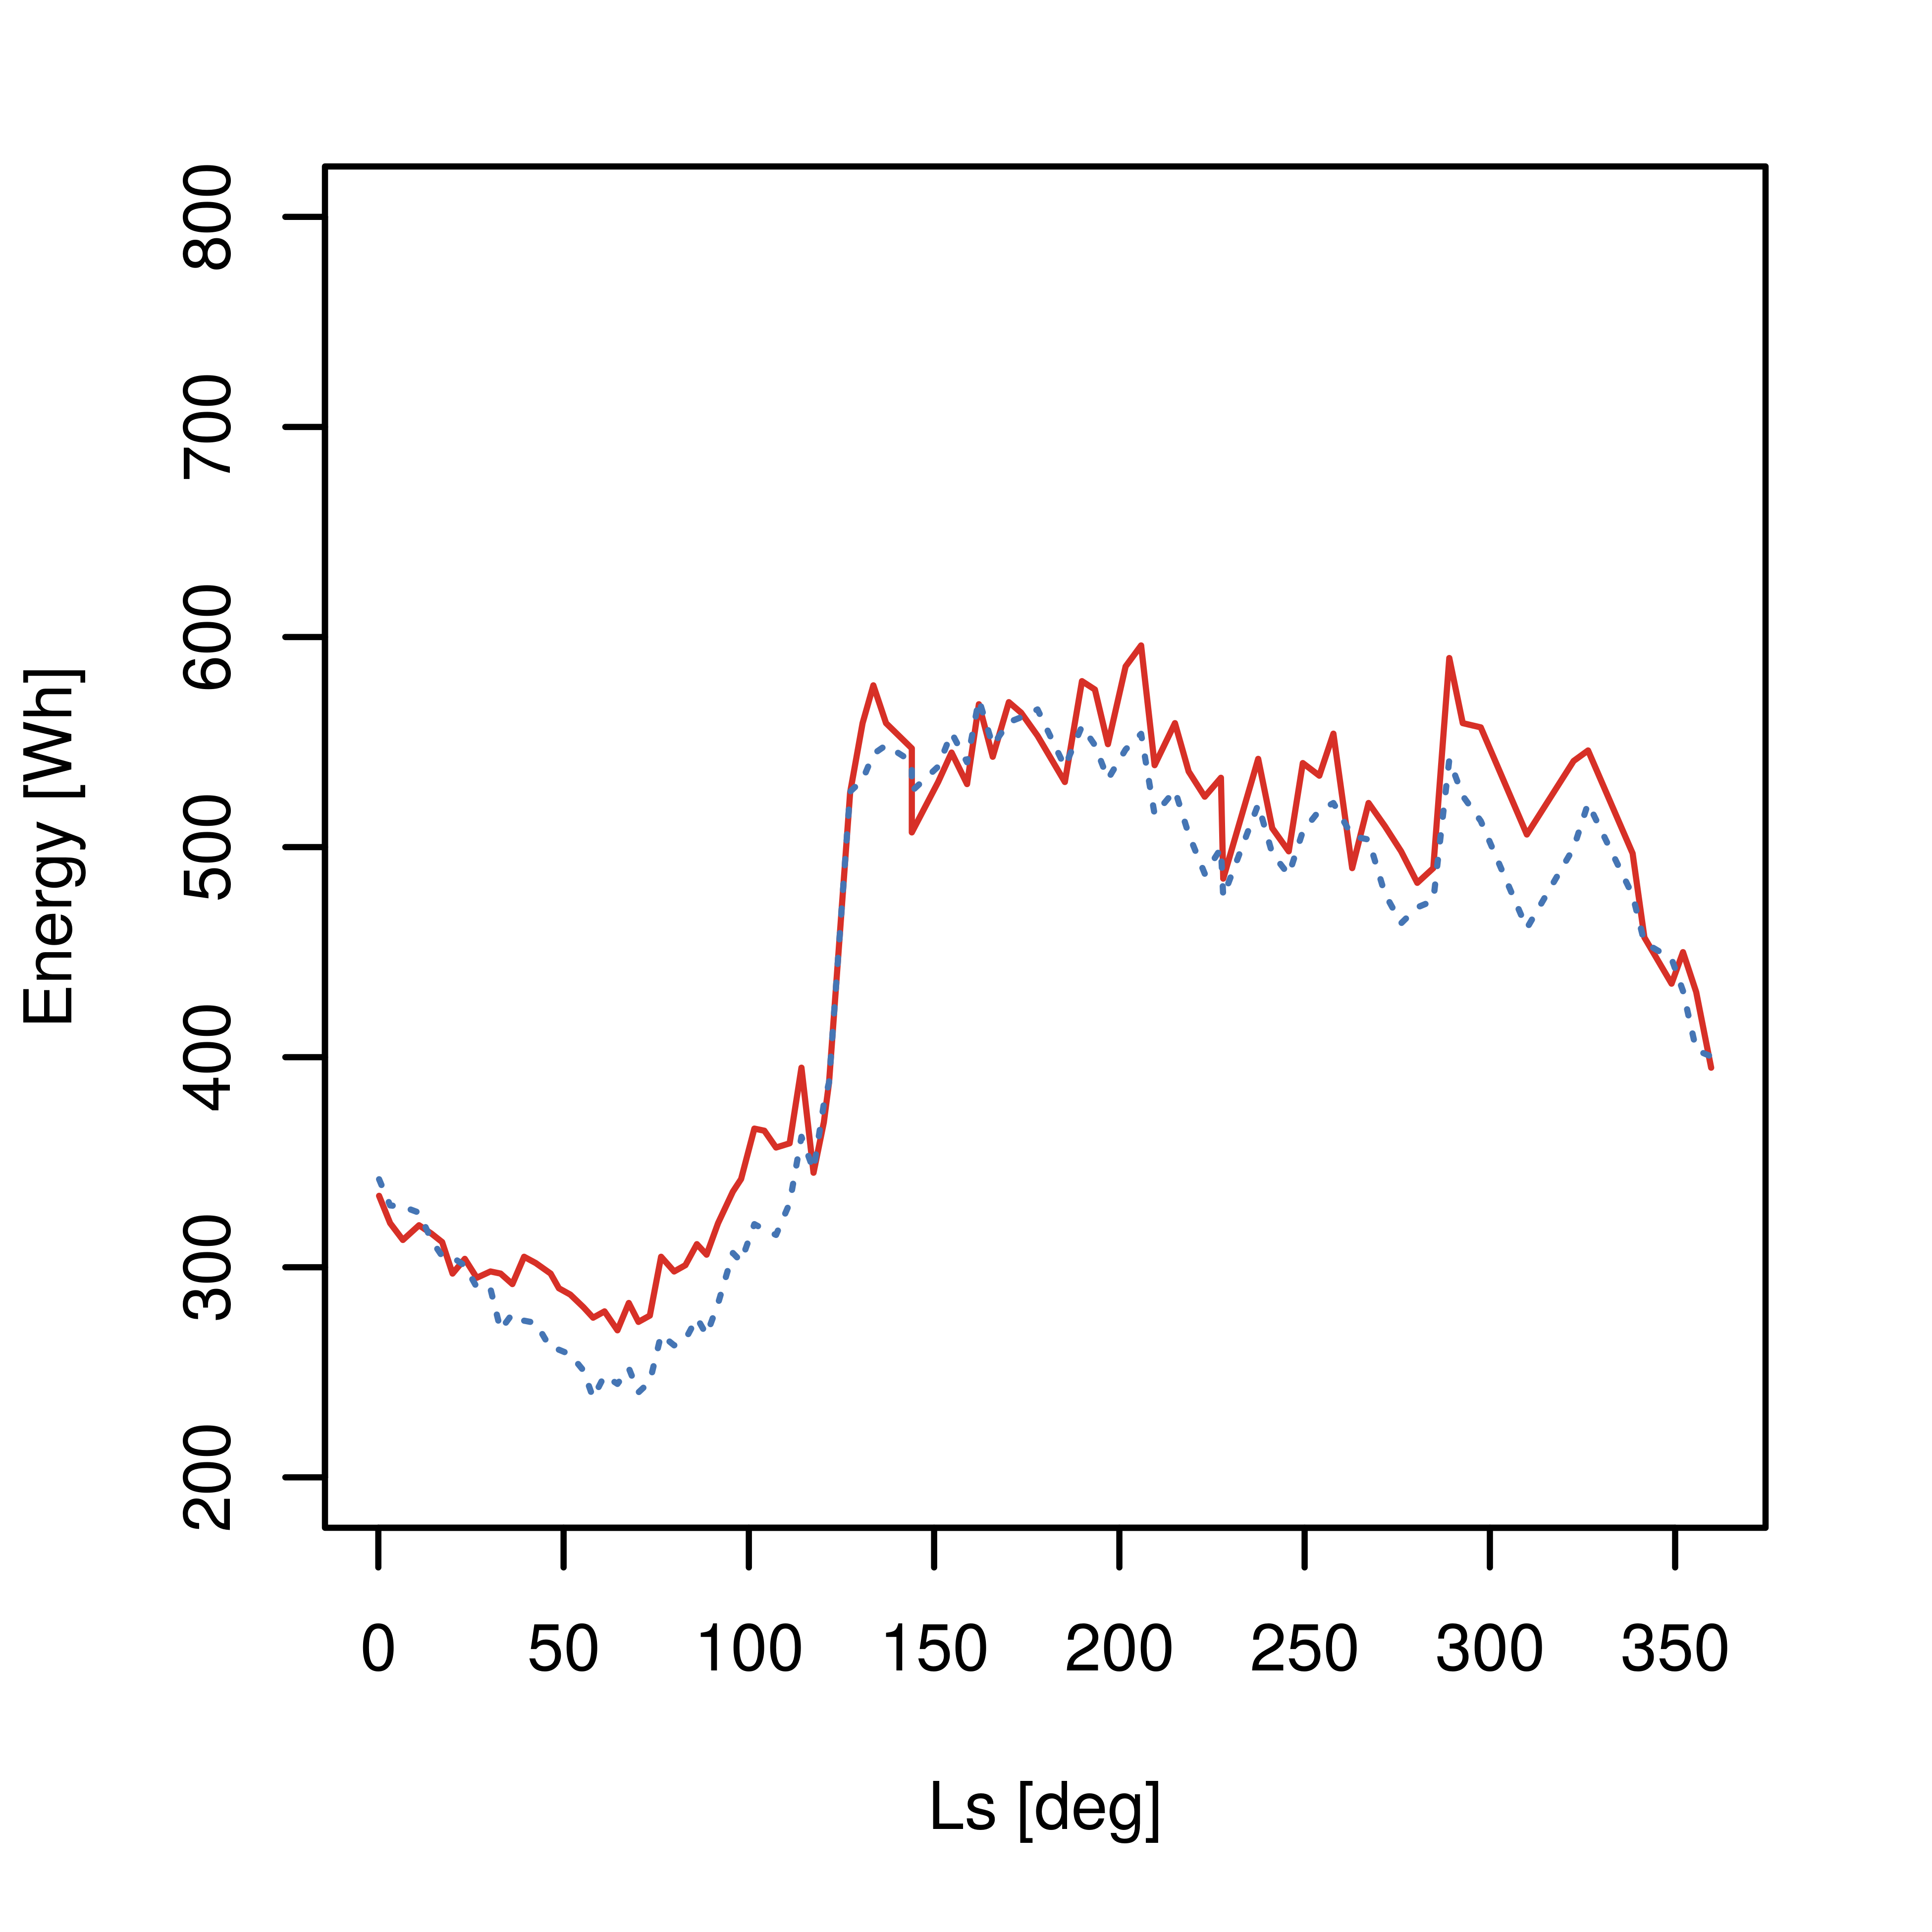
\includegraphics[height=\graphicsHeight]{sections/appendix/energy-error-margin/plots/predicted-vs-measured-energy-my30-adjusted-without-outliers.png}
		\subcaption{MY30 (outliers ignored)}
		\label{fig:plot:sub:mer-energy-production-predicted-vs-reported-my30-adjusted-without-outliers}
	\end{subfigure}\hfill
    \begin{subfigure}[t]{\subfigureWidth}
        \centering
		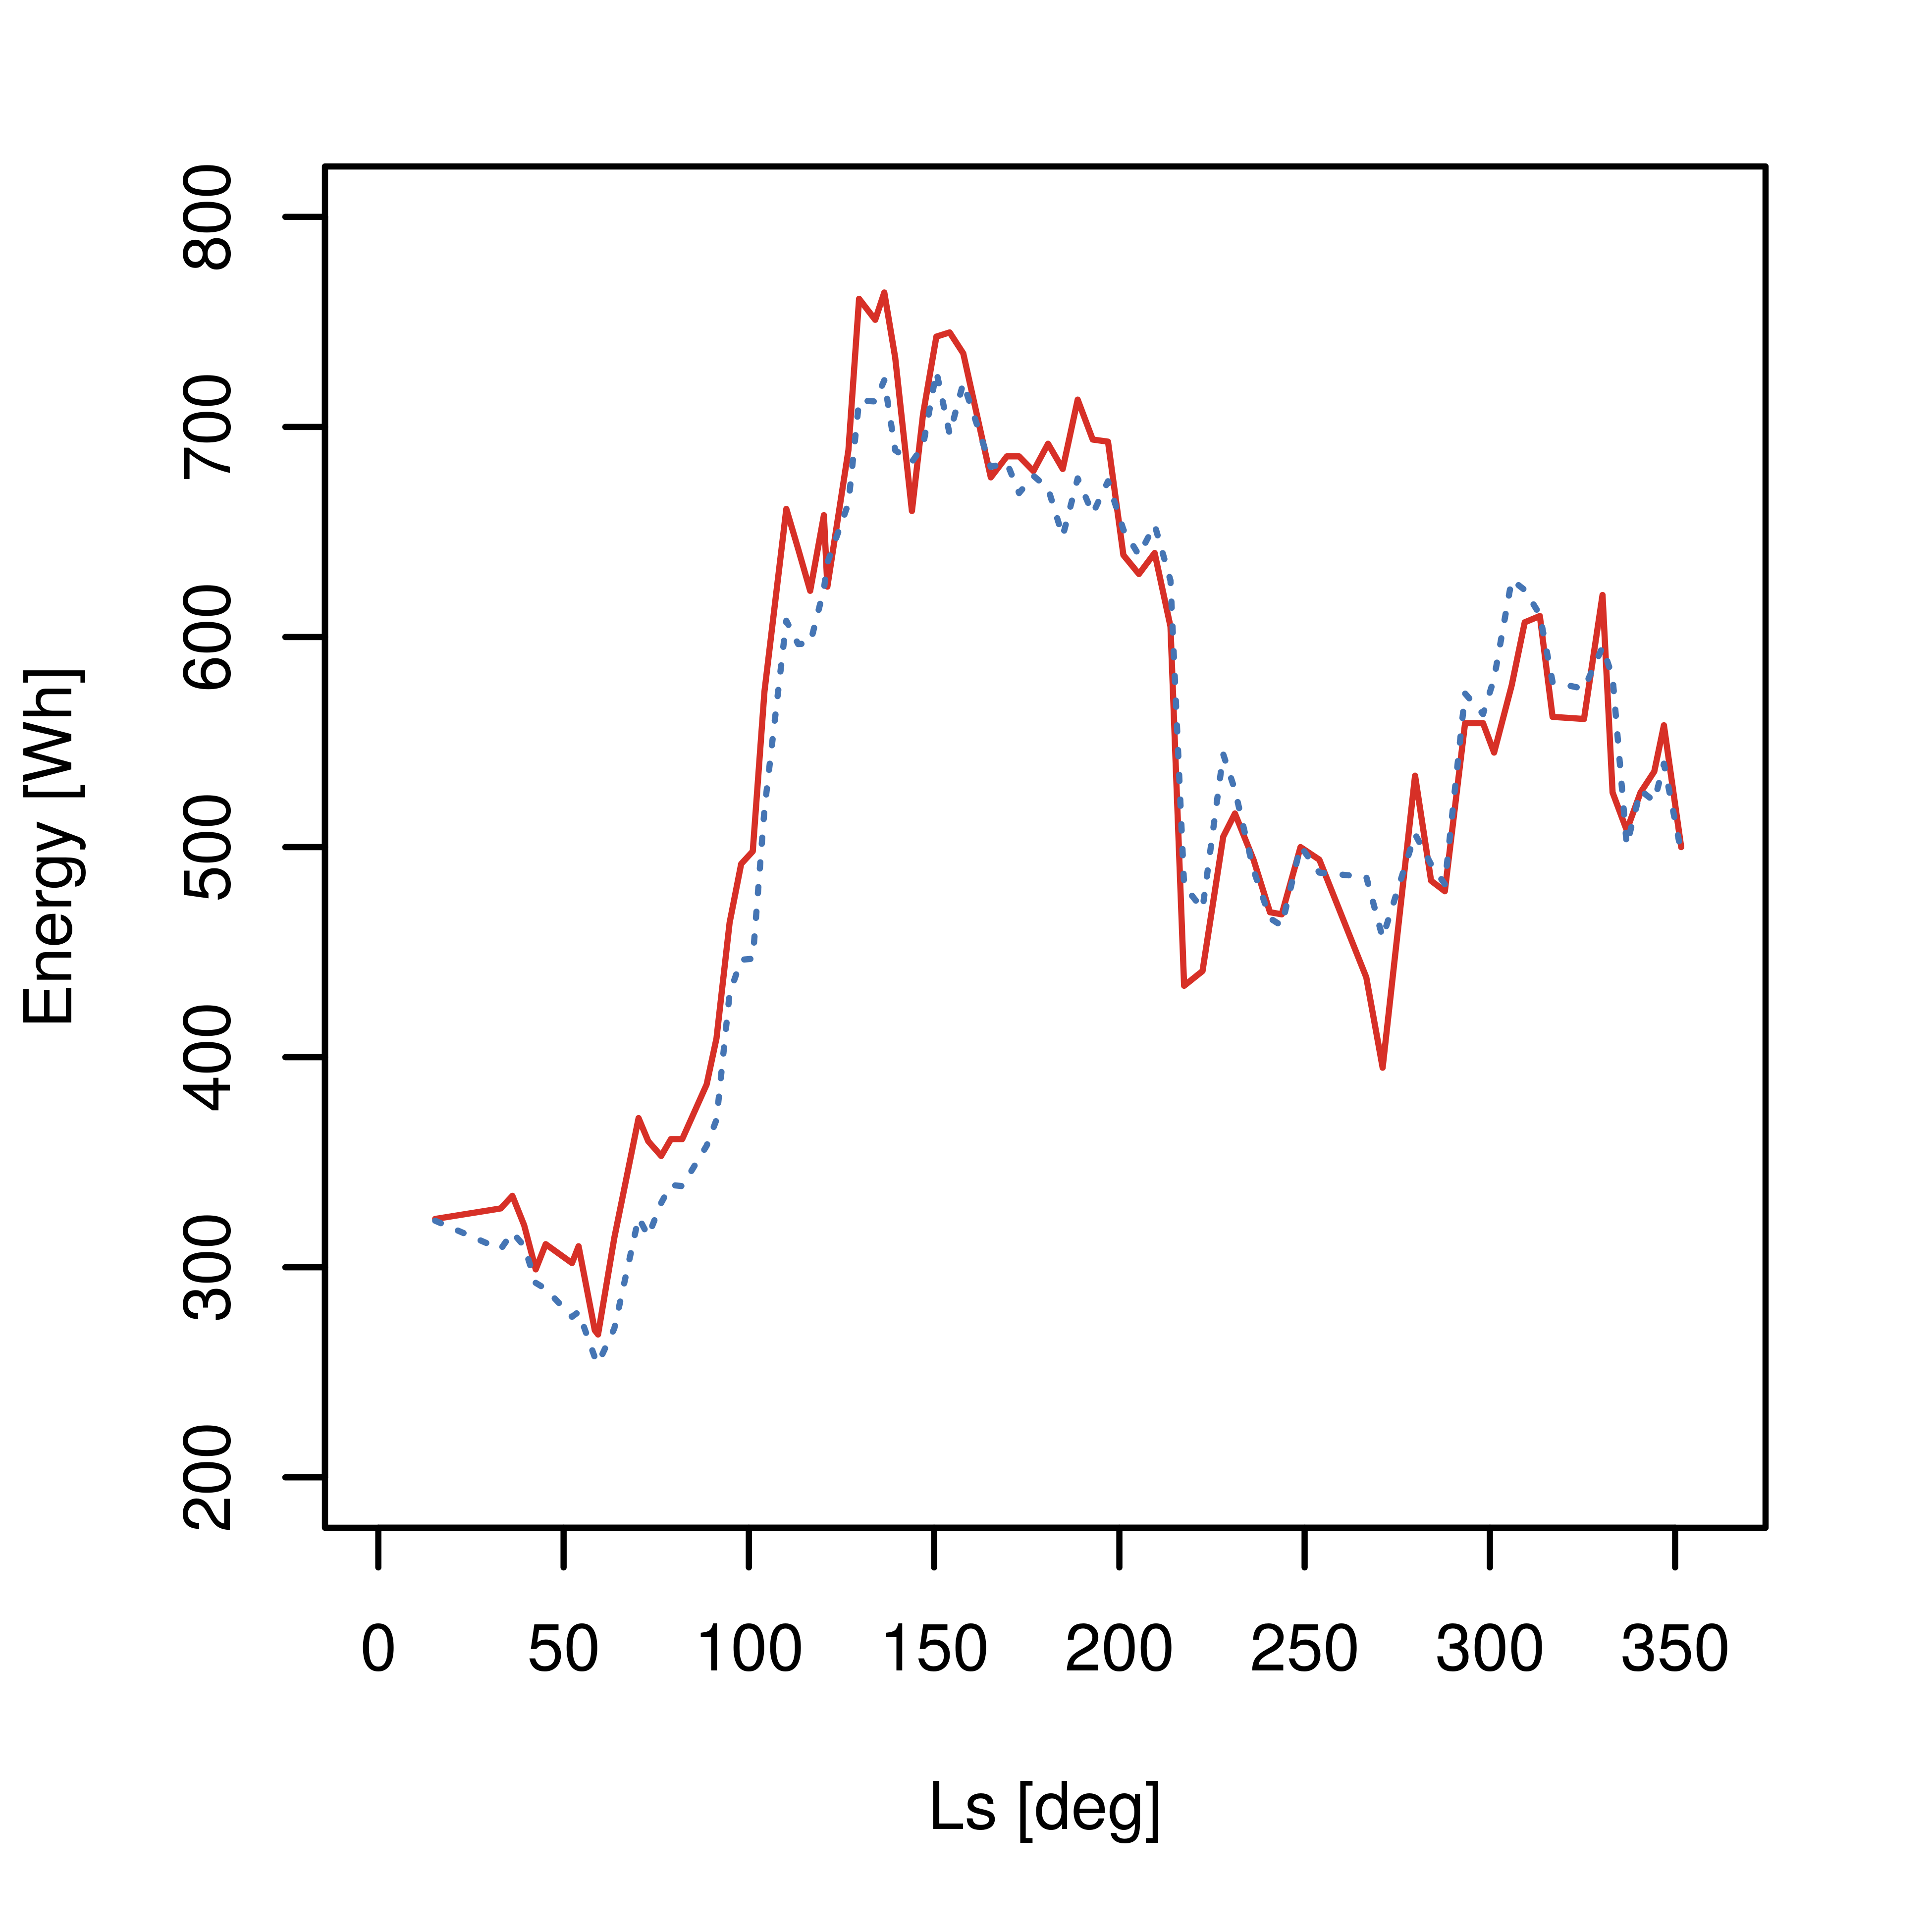
\includegraphics[height=\graphicsHeight]{sections/appendix/energy-error-margin/plots/predicted-vs-measured-energy-my32-adjusted-without-outliers.png}
		\subcaption{MY32 (outliers ignored)}
		\label{fig:plot:sub:mer-energy-production-predicted-vs-reported-my32-adjusted-without-outliers}
	\end{subfigure}
    \caption[Opportunity energy production: adjusted prediction versus reported]
            {Opportunity energy production: adjusted prediction versus reported. The predicted lines across the first row are obtained with iteratively determined calculation adjustments that narrowed the calculated predicted values' error margin range from \SI{-33}{\percent}/+\SI{7}{\percent} to \SI{-10}{\percent}/+\SI{25}{\percent}. The second row is obtained in a similar fashion but with divergence outliers ignored in order to further narrow the error margin range to \SI{-11}{\percent}/+\SI{5}{\percent}.}
    \label{fig:plot:mer-energy-production-predicted-vs-reported-adjusted-with-and-without-outliers}
\vspace{-2ex}
\end{figure}
